\subsection*{2.1}
Refer to Figure \ref{fig:part2_1}
\begin{figure}[]
	\caption{Plot of raw seismic data}
	\label{fig:part2_1}
	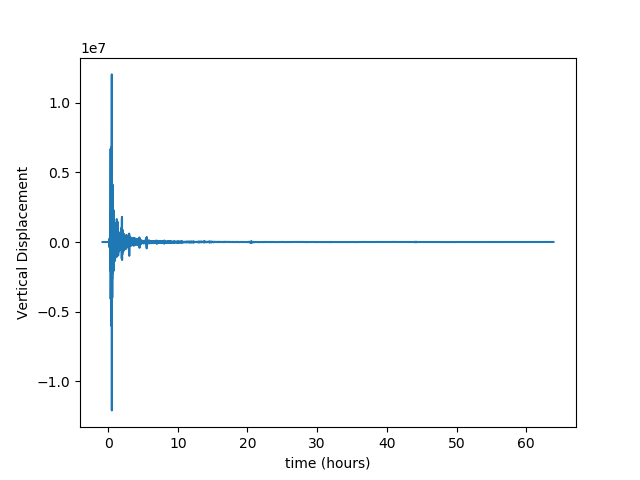
\includegraphics[width=\linewidth]{figures/part2_1.png}
\end{figure}

\subsection*{2.2}
Refer to Figure \ref{fig:part2_2}
\begin{figure}[]
	\caption{Power spectrum of raw data without windowing}
	\label{fig:part2_2}
	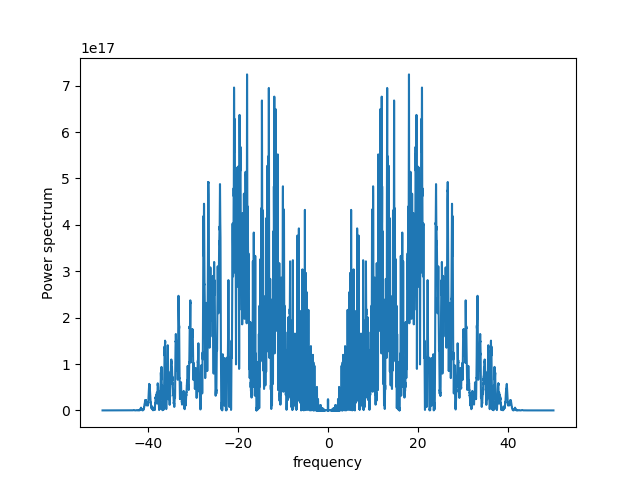
\includegraphics[width=\linewidth]{figures/part2_2.png}
\end{figure}

\subsection*{2.3}
Refer to Figure \ref{fig:part2_3}
\begin{figure}[]
	\caption{Power spectrum of raw data after detrending and applying hanning window}
	\label{fig:part2_3}
	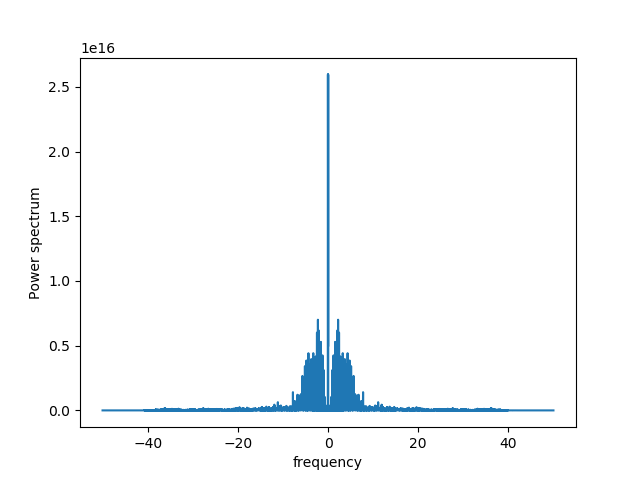
\includegraphics[width=\linewidth]{figures/part2_3.png}
\end{figure}

\subsection*{2.4}
Refer to Figure \ref{fig:part2_4}
\begin{figure}[]
	\caption{Plots in Figures \ref{fig:part2_2} and \ref{fig:part2_3} overlayed and zoomed in}
	\label{fig:part2_4}
	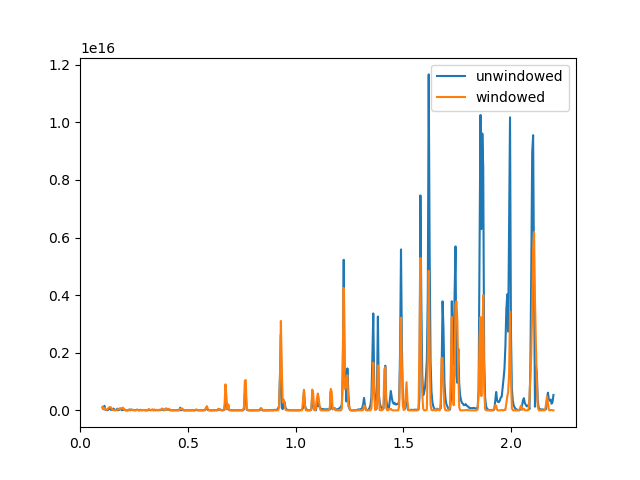
\includegraphics[width=\linewidth]{figures/part2_4.png}
\end{figure}


\subsection*{2.5}
Refer to Figure \ref{fig:part2_5}
\newpage
\begin{landscape}
\begin{figure}[]
	\caption{Identification of normal modes from power spectra of seismic data}
	\label{fig:part2_5}
	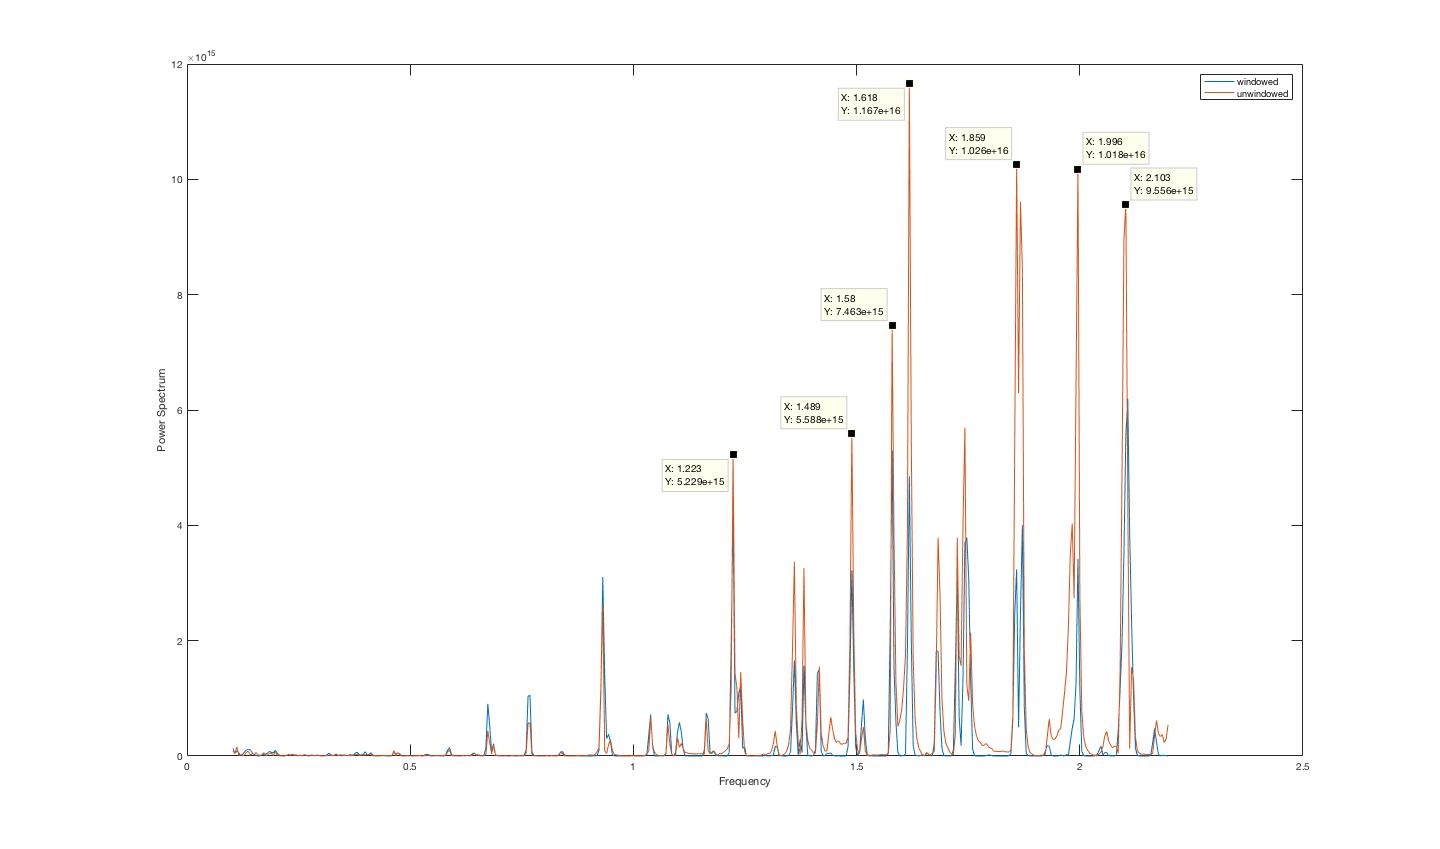
\includegraphics[width=\linewidth]{figures/part2_5.png}
\end{figure}
\end{landscape}
\newpage